% TEMPLATE for Usenix papers, specifically to meet requirements of
%  USENIX '05
% originally a template for producing IEEE-format articles using LaTeX.
%   written by Matthew Ward, CS Department, Worcester Polytechnic Institute.
% adapted by David Beazley for his excellent SWIG paper in Proceedings,
%   Tcl 96
% turned into a smartass generic template by De Clarke, with thanks to
%   both the above pioneers
% use at your own risk.  Complaints to /dev/null.
% make it two column with no page numbering, default is 10 point

% Munged by Fred Douglis <douglis@research.att.com> 10/97 to separate
% the .sty file from the LaTeX source template, so that people can
% more easily include the .sty file into an existing document.  Also
% changed to more closely follow the style guidelines as represented
% by the Word sample file. 

% Note that since 2010, USENIX does not require endnotes. If you want
% foot of page notes, don't include the endnotes package in the 
% usepackage command, below.

% This version uses the latex2e styles, not the very ancient 2.09 stuff.
\documentclass[letterpaper,twocolumn,10pt]{article}
\usepackage{usenix,epsfig,endnotes}
\usepackage{subfigure}
\usepackage{color}
\usepackage{array}
\usepackage{longtable}
\usepackage{calc}
\usepackage{multirow}
\usepackage{hhline}
\usepackage{ifthen}
\usepackage{url}
\begin{document}

%don't want date printed
\date{}

%make title bold and 14 pt font (Latex default is non-bold, 16 pt)
\title{\Large \bf Preserving Interactivity of GUI Applications}

%for single author (just remove % characters)
\author{
{\rm Hilfi Alkaff}\\
hilfialkaff@berkeley.edu
\and
{\rm Vu Chiem}\\
vuchiemh@berkeley.edu
\and
{\rm Andrew Wang}\\
awang@eecs.berkeley.edu
% copy the following lines to add more authors
% \and
% {\rm Name}\\
%Name Institution
} % end author

\maketitle

% Use the following at camera-ready time to suppress page numbers.
% Comment it out when you first submit the paper for review.
\thispagestyle{empty}


\subsection*{Abstract}
The manycore machines of the future will likely run a diverse set of concurrent workloads, placing additional demands on resource allocation and scheduling policies of the operating system to ensure interactive behavior of user applications while running high throughput batch processing jobs in the background. In our paper, we show that a degree of performance isolation can be achieved on Linux through the use of the existing CPUSET mechanism for realistic GUI applications.

\section{Introduction}

Motivation: existing schedulers do a poor job running simultaneous workloads with similar resource requirements and different interactive requirements. What we want is performance isolation.

Tessellation / Decomposition into the Cell model


More fascinating text. Features\endnote{Remember to use endnotes, not footnotes!} galore, plethora of promises.\\

\section{Related Work}

Things that should be mentioned here:
\begin{enumerate}
\item Linux schedulers: Redline, AIRS
\item mClock ?
\item fos, Barrelfish, Corey
\item Lithe: user level scheduler that is more hardware thread aware
\end{enumerate}

Some embedded literal typset code might 
look like the following :

\section{Implementation}
\subsection{Channels}
We should mention these things in this section:
\begin{enumerate}
\item Lock free mechanism
\item Single consumer/producer
\item Loose measurement details (throughput for small message size)
\item Shared memory
\item Signalling mechanism
\end{enumerate}

Channel is the only communication mechanism that is being used in our system. We build this by re-implementing the existing non-blocking buffer~\cite{Kim:2007:EAN:1260991.1261857} on top of Linux shared memory segments. All of the channels, except the nameserver's which is going to be discussed later, is lock-free so as to minimize the overhead of lock contention as much as possible and thereby increasing the throughput.

This communication mechanism is point-to-point too. The way one entity inform the other that data has been to their side is by the UNIX signalling mechanism. For simplicity purpose, the entity neither do any combination of polling and interrupt nor polling mechanism although that will certainly add a considerable amount of overhead in the system.


\subsection{Nameserver}
The nameserver functions similarly to a DNS server for channel IPC. It allows services to register themselves under an ASCII string {\tt name}, which can then be used in other applications and services. When a subsequent request is placed for this {\tt name}, the nameserver initializes a new channel and sends the shared memory ID to both processes. Further communication between the server and client happen without further nameserver intervention.

There is a slight chicken and egg problem here, since an application needs to already have a channel open to the nameserver before it can request channels to be opened. This is handled by reserving a globally known channel purely for this initialization step; applications will get a lock, inform the nameserver of its presence, wait for the nameserver to allocate a new channel for the two of them, and then unlock and continue communication on the new channel. Since this initialization channel is only used once by each process, there is little lock contention.

\subsection{Qt Embedded}
\begin{enumerate}
\item Framebuffer
\item Porting to tessellation
\item Client/server model
\item Decomposition
\end{enumerate}

Since this project is largely motivated by Tesselation OS~\cite{liu09tessellation, tessellation-hotpar10}, we would like to be able to port our design to the code base of Tesselation. It will be easier to do so with Qt Embedded since the it is not as complicated and large as, say, X/X11 stack. Not only that, it will also be harder to promise the resource guarantees if the GUI service has a number of layers embedded within.

Fortunately for us, Qt's client/server model is decomposed in a way similar to Tesselation's and also, its code is very modularized. Hence, it's less harder in our part to find out which part of Qt that we should modify. 

What happens in the internals of Qt is that, there is already a client and server, as mentioned earlier. The default communication mechanism that is being used here is tcp socket. Whenever the client wants to display an animation, it will notify the server that it would like to to do so. After a few messages have been exchanged and agreement has been reached, the server will assign the client its entitled share of the framebuffer which the client could use it as much as it likes for displaying the animation.

Additionally, when there's an I/O input (e.g. mouse or keyboard), the server will be immediately notified of it and does some processing and/or filtering before forwarding it to the appropriate client. 

\subsection{Resource Allocation Daemon}

The purpose of resource allocation daemon is to provide any services and clients with whatever hardware resources that they are requesting. One type of resource that all clients and services will need is CPU. This is one of the first things that the clients and the systems will have to request for.

One point to note here is that the client will not request, say, a guaranteed portion of the graphic driver directly to the resource allocation daemon. It's actually the service will request a big portion of this resource. Then, the client will request its portion of this resource from the service to do whatever the client wants. 

There is a huge possibility of separating the policy from the mechanism in our system. In that case, different priorities could be assigned to the clients and a client who has a higher priority will be entitled to more share of the resources. However, due to time constraints, we leave this possibility for future work

\section{Evaluation}

% you can also use the wonderful epsfig package...
\begin{figure*}[t]
  \begin{center}
    \subfigure[Sunspider JS benchmark]{\label{fig:edge-a}\includegraphics[scale=0.75]{sunspider.ps}}
    \subfigure[Textedit latency measurements]{\label{fig:edge-b}\includegraphics[scale=0.75]{textedit.ps}} \\
  \end{center}
  \caption{Comparison between unmodified and channels-based versions of Qt}
  \label{fig:benchmarks}
\end{figure*}

\subsection{Test setup}

The test harness used was a commodity desktop PC with a quad core Intel i7-870 processor clocked at 2.93 GHz and 4GB of RAM. Hyperthreading, Turbo Boost, and power saving states were all disabled to normalize the performance of the CPU cores. Loaded conditions were simulated by running 128 CPU-bound background threads. This number is somewhat arbitrary, but a lower or higher number of threads would likely result in a proportional change without effecting the meaning of our results.

We encountered difficulties in getting both the modified and unmodified version of Qt to run correctly on an actual framebuffer. As a substitute, all tests were run on the Qt Embedded virtual framebuffer, an X11 application. This means there are additional layers of software, such as X11 and the WM, that interpose between user input and the I/O server. However, our timings are done above these layers, and we believe that this favors neither the unmodified nor channels-based version of Qt.

\subsection{Channels}

To show that our channel implementation was not bottlenecking our Qt applications, we wrote a variety of stress test and benchmarking suites to test latency, throughput, and correctness. Profiling of client / service communication revealed that vast majority of messages were small (4-24 bytes) with a few that were substantially larger (24-200 bytes). As shown in Table \ref{tab:channel_latency}, our channel implementation handles sending these types of messages with latency in the range of microseconds. The rate at which Qt sends messages is also rather low, but our channels implementation can easily push ??? MB/s even for small 4 byte messages (Table \ref{tab:channel_tput}).

\begin{table}[tp]
\caption{Channel Latency}
\label{tab:channel_latency}
\centering
\begin{tabular}{|l | l | l | l |}
\hline
		&Latency ($\mu$s)	&Median	&Std dev\\ \hline
4B		&0.14	&0.13	&0.049\\
64B		&30.60	&16.67	&37.24\\
128B	&0.16	&0.18	&0.033\\
512B	&0.26	&0.15	&0.42\\
\hline
\end{tabular}
\end{table}

\begin{table}[tp]
\caption{Channel Throughput (MB/s)}
\centering
\label{tab:channel_tput}
\begin{tabular}{|l | l | l | l | l |}
\hline
			&4B 	& 64B	& 128B	& 512B \\ \hline
Throughput	&0.26	&0.15	&0.42	& 0.42 \\
\hline
\end{tabular}
\end{table}


\subsection{Web Browser}

The first user application we chose for testing was a simple Qt web browser based on WebKit. Browsers are probably one of the most commonly used and installed user applications, making a browser a representative choice as a "real world" application. Browsers also have the benefit of a wide variety of Javascript benchmark suites, such as SunSpider~\cite{sunspider}, Kraken~\cite{kraken}, and V8~\cite{v8benchmark}.

We chose to use Apple's SunSpider JS benchmark, which is mostly CPU-bound. Figure \ref{fig:benchmarks} shows the time to complete SunSpider, lower being better. In the no load case, the unmodified version of Qt performs roughly three times faster than our version. This is somewhat disappointing; our current guess is that signal handling within the channels is triggering a large number of context switches.

However, the tables are turned in the loaded situation. Our version of Qt maintained roughly equivalent performance, while the unmodified version's performance degraded by more than a factor of 20 (and 7 times worse than our version). This is due to the performance isolation guaranteed by CPUSETs and the resource allocation daemon; Qt-C is guaranteed its allocation of the CPU even under load, while Qt has to share the CPU with other tasks and experiences additional scheduling and context switching overhead.

\subsection{Textedit}

To illustrate interactivity in our experiments, we use Qt sample textedit program and one of us will mash the keyboard and mouse for a couple of minutes and the latency between when the keyboard is pressed until when the change is reflected in the screen is measured. We also ensure that the events (i.e. keyboard or mouse pressed event) that are received in the server are all forwarded to the clients. Thus, our implementation is very reliable since it doesn't drop any of the registered events. 

Figure \ref{fig:benchmarks} shows that our implementation loses to Qt performance-wise under no load. One speculation that we made to explain this difference is that we never use polling like the original Qt does and only use interrupts in our channel implementation. The overhead due to the frequent use of interrupts will be quite significant. 

With load running in the background the performance of our implementation almost does not change as promised by our guarantees, while the original implementation of Qt performs a lot worse. Finding out the work done by the background thread is outside the scope of this paper since what we are promising is that the GUI applications are able to run smoothly and not how much work is loss by the background threads. We expect the work done to be much lower in our case though, since we reserve a subset of our cores for our system services and the applications. 

\begin{table}[htp]
\caption{Textedit interactivity}
\label{tab:textedit_table}
\centering
\begin{tabular}{|l | l | l | l |}
\hline
	&Latency ($\mu$s)	&Median	&Std dev\\ \hline
Qt, NL	&0.14	&0.13	&0.049\\
Qt, L	&30.60	&16.67	&37.24\\
Qt-C, NL	&0.16	&0.18	&0.033\\
Qt-C, L	&0.26	&0.15	&0.42\\
\hline
\end{tabular}
\end{table}

\section{Conclusion}

A polite author always includes acknowledgments.  Thank everyone,
especially those who funded the work. 

\section{Availability}

It's great when this section says that MyWonderfulApp is free software, 
available via anonymous FTP from

\begin{center}
{\tt ftp.site.dom/pub/myname/Wonderful}\\
\end{center}

Also, it's even greater when you can write that information is also 
available on the Wonderful homepage at 

\begin{center}
{\tt http://www.site.dom/\~{}myname/SWIG}
\end{center}

\footnotesize{\bibliographystyle{acm}
\bibliography{bibliography}}

\theendnotes

\end{document}
